\chapter{Introducción}
\label{cap:introduccion}

% Según la normativa  para Trabajos de Fin de Grado\footnote{\url{https://informatica.ucm.es/file/normativatfg-2021-2022?ver} (ver versión actualizada para cada curso académico)}, la memoria incluirá una portada normalizada con la siguiente información: título en castellano, título en inglés, autores, profesor director, codirector si es el caso, curso
% académico e identificación de la asignatura (Trabajo de fin de grado del Grado en -
% nombre del grado correspondiente-, Facultad de Informática, Universidad Complutense de Madrid). Los datos referentes al título y director (y codirector en su caso) deben corresponder a los publicados en la página web de TFG.

% La memoria debe incluir la descripción detallada de la propuesta hardware/software realizada y ha de contener:
% \begin{enumerate}
% \renewcommand{\theenumi}{\alph{enumi}}
	% \item un índice,
	% \item un resumen y una lista de no más de 10 palabras clave para su búsqueda % bibliográfica, ambos en castellano e inglés,
	% \item una introducción con los antecedentes, objetivos y plan de trabajo,
	% \item resultados y discusión crítica y razonada de los mismos, con sus % conclusiones,
	% \item bibliografía.
% \end{enumerate}
% Para facilitar la escritura de la memoria siguiendo esta estructura, el estudiante podrá usar las plantillas en LaTeX o Word preparadas al efecto y publicadas en la página web de TFG.

% La memoria constará de un mínimo de 25 páginas para los proyectos realizados por un único estudiante, y de al menos 5 páginas más por cada integrante adicional del grupo. En este número de páginas solo se tiene en cuenta el contenido correspondiente a los apartados c y d del punto anterior.

% La memoria puede estar escrita en castellano o inglés, pero en el primer caso la introducción y las conclusiones deben aparecer también en inglés. Las memorias de los TFG matriculados en el grupo I deberán estar escritas íntegramente en inglés, excepto por lo especificado en los puntos 1 y 2 anteriores (título, resumen y lista de palabras clave).

% En caso de trabajos no unipersonales, cada participante indicará en la memoria su contribución al proyecto con una extensión de al menos dos páginas por cada uno de los participantes.

% Todo el material no original, ya sea texto o figuras, deberá ser convenientemente citado y referenciado. En el caso de material complementario se deben respetar las licencias y \emph{copyrights} asociados al software y hardware que se emplee. En caso contrario no se autorizará la defensa, sin menoscabo de otras acciones que correspondan.


\section{Motivación}
La principal motivación por la que hemos decidido hacer este proyecto es que, según ~\cite{wearesocial2024}, se mueven un gran volumen de datos en redes sociales (medible en la escala de exabytes), tienen una gran cantidad de usuarios, superando los 5 mil millones de usuarios activos y un tiempo medio de uso de 2 horas y 23 minutos al día, pero nos mantenemos 6 horas y 40 minutos en línea de media diariamente. Además, la red social más utilizada en 2024 fue TikTok, la cual se basa en videos de corta duración, admitiendo en sus orígenes videos de hasta 60 segundos y actualmente hasta 60 minutos. Esto hace que el paso de información secreta a través de vídeos con audio en la red pública pase desapercibido debido a su abusivo pero común uso en la actualidad. 

\begin{figure}[h]
	\centering
	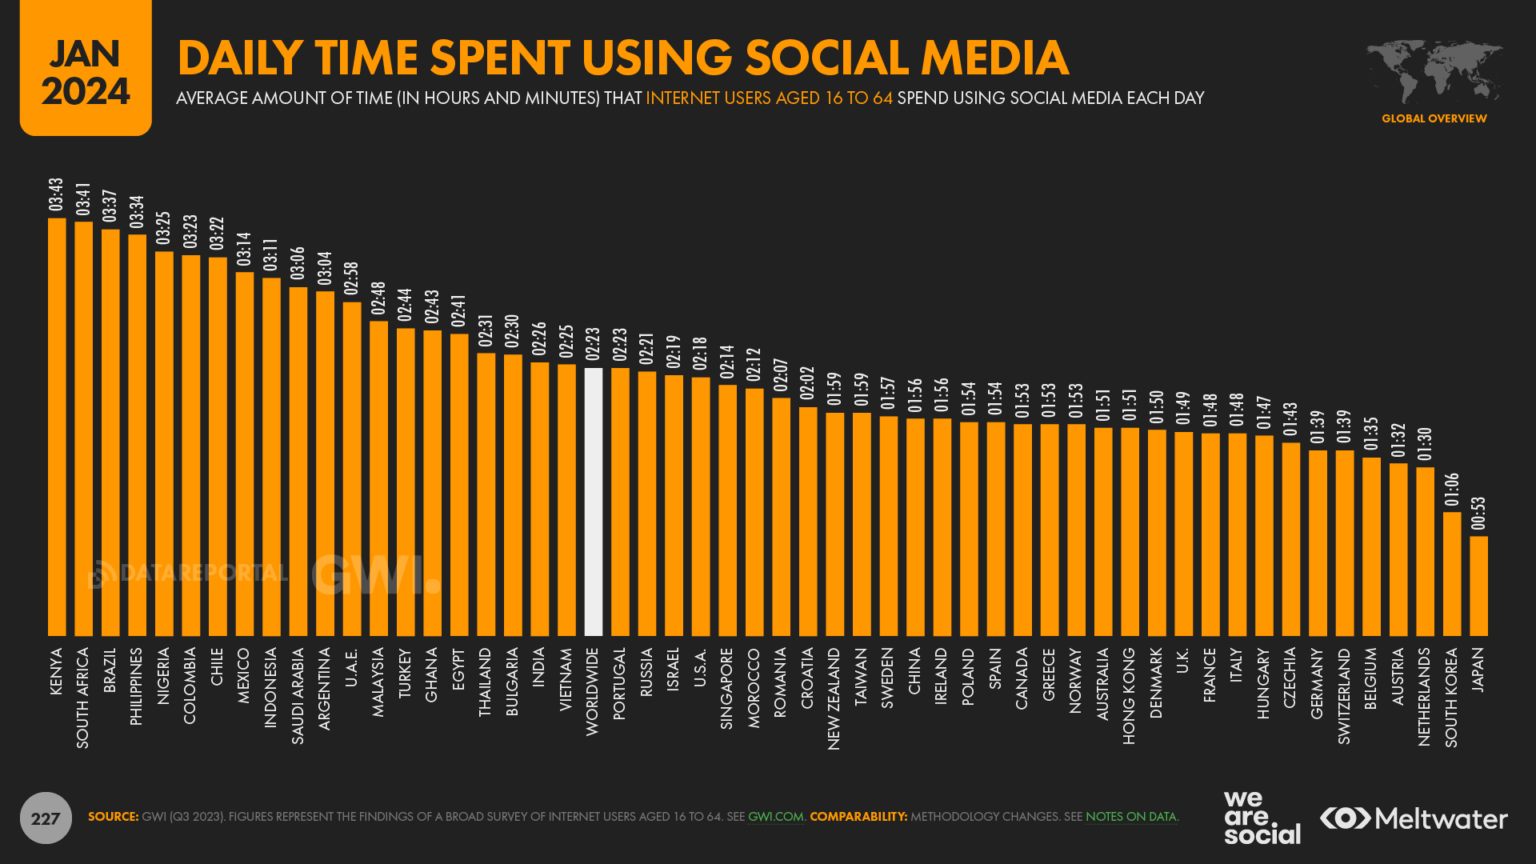
\includegraphics[width = 0.8\textwidth]{Imagenes/pitea/grafica_tiempo_redes_sociales.png}
	\caption[Uso de redes sociales por país.]{Gráfica del  tiempo de uso de redes sociales por país. ~\cite{wearesocial2024}.}
	\label{fig:proceso}
\end{figure}


Para evitar riesgo de confidencialidad en los datos, se vuelve fundamental el uso de la esteganografía, que será introducida con más detalle en este documento pero por ahora la definiremos como técnicas de ocultación de información, para garantizar que, si alguien obtiene un video de manera lícita o ilícita, no sea capaz de detectar que contiene información valiosa, debido a que ésta está oculta y aparenta ser un video más en el mar de bytes.


\section{Objetivos}
\label{sec:ob}
El objetivo de este proyecto es desarrollar una herramienta capaz de utilizar métodos de transformación de texto a imágenes y de imágenes a audio con el fin de transmitir información de manera oculta y aprovechar el intenso uso de las redes sociales que hay en la actualidad.

Para ello, nos centraremos en:

\begin{itemize}
    \item Creación de una CLI (\textit{Command-line interface}).
    \item Implementación de algoritmos para la ocultación y desocultación tanto de texto en imagen como de imagen en audio.
    \item Tratamiento de ondas acústicas en la informática.
    \item Uso de criptografía de clave secreta.
\end{itemize}


\section{Plan de trabajo}
\label{sec:trab}
En esta sección se describe el plan de trabajo detallado con el que se espera alcanzar los objetivos del proyecto. 

\subsection{Etapa 1: Investigación previa }
\label{subsec:1}

\textbf{Objetivo:} Realizar una investigación previa al desarrollo de la herramienta con el fin de situarse en los conocimientos y técnicas necesarias.\\

\textbf{Tareas:}
\begin{itemize}
    \item Búsqueda de información sobre esteganografía y criptografía.
    \item Búsqueda de información sobre la codificación de archivos multimedia.
    \item Análisis de las herramientas existentes.
\end{itemize}



\subsection{Etapa 2: Desarrollo de un prototipo funcional básico}
\label{subsec:2}
\textbf{Objetivo:} Crear un prototipo funcional de la herramienta que realice la ocultación y desocultación mediante LSB \textit{(Less Significant Bit)}.\\

\textbf{Tareas:}
\begin{itemize}
    \item Desarrollar un programa secuencial que realice el proceso completo de ocultar y desocultar.
    \item Implementar las funcionalidades básicas, como cifrar el texto mediante AES y ocultar el texto y la imagen mediante el método de ocultación LSB.
    \item Realizar pruebas para verificar que el sistema básico funcione correctamente y la información no se modifica en el proceso.
\end{itemize}



\subsection{Etapa 3: Modularización y ampliación de funcionalidades}
\label{subsec:3}
\textbf{Objetivo:} Modularizar el programa y añadir funcionalidades adicionales, como generar audios a partir de las imágenes para transmitirlos por SSTV.\\

\textbf{Tareas:}
\begin{itemize}
    \item Dividir el código en módulos haciendo un uso apropiado de la POO (Programación Orientada a Objetos) para separar las responsabilidades de cifrado, esteganografía en imágenes, esteganografía en audio y manejo de entradas y salidas.
    \item Implementar funcionalidades adicionales, como la capacidad de elegir entre diferentes técnicas de ocultación.
    \item Realizar pruebas de integración para asegurarse de que los módulos funcionan bien juntos.
\end{itemize}

\subsection{Etapa 4: Creación de la CLI}
\label{subsec:4}
\textbf{Objetivo:} Crear la interfaz de línea de comandos para facilitar la interacción con el programa.\\

\textbf{Tareas:}
\begin{itemize}
    \item Implementar la interfaz de línea de comandos.
    \item Integrar la interfaz con los módulos desarrollados previamente.
    \item Asegurar que los usuarios solo puedan elegir flujos posibles de ejecución.
\end{itemize}

\subsection{Etapa 5: Pruebas de la herramienta}
\label{subsec:5}
\textbf{Objetivo:} Realizar pruebas sobre la herramienta para asegurar la fiabilidad y descubrir las limitaciones del sistema.\\

\textbf{Tareas:}
\begin{itemize}
    \item Realizar pruebas para comprobar la fiabilidad de la herramienta empleándola en casos reales de uso.
    \item Realizar pruebas para estudiar las limitaciones de la herramienta.
\end{itemize}


\subsection{Etapa 6: Documentación}
\label{subsec:6}
\textbf{Objetivo:} Documentar la arquitectura de la herramienta así como las conclusiones a las que hemos llegado.\\


\textbf{Tareas:}
\begin{itemize}
    \item Crear documentación detallada sobre el código, las funcionalidades, el uso de la herramienta, la instalación de esta, las tecnologías usadas y también las descartadas.
    \item Preparar una presentación para mostrar el proyecto y sus resultados finales.
\end{itemize}


% \section{Explicaciones adicionales sobre el uso de esta plantilla}
% Si quieres cambiar el \textbf{estilo del título} de los capítulos del documento, edita el fichero \verb|TeXiS\TeXiS_pream.tex| y comenta la línea \verb|\usepackage[Lenny]{fncychap}| para dejar el estilo básico de \LaTeX.

% Si no te gusta que no haya \textbf{espacios entre párrafos} y quieres dejar un pequeño espacio en blanco, no metas saltos de línea (\verb|\\|) al final de los párrafos. En su lugar, busca el comando  \verb|\setlength{\parskip}{0.2ex}| en \verb|TeXiS\TeXiS_pream.tex| y aumenta el valor de $0.2ex$ a, por ejemplo, $1ex$.

% TFGTeXiS se ha elaborado a partir de la plantilla de TeXiS\footnote{\url{http://gaia.fdi.ucm.es/research/texis/}}, creada por Marco Antonio y Pedro Pablo Gómez Martín para escribir su tesis doctoral. Para explicaciones más extensas y detalladas sobre cómo usar esta plantilla, recomendamos la lectura del documento \texttt{TeXiS-Manual-1.0.pdf} que acompaña a esta plantilla.

% El siguiente texto se genera con el comando \verb|\lipsum[2-20]| que viene a continuación en el fichero .tex. El único propósito es mostrar el aspecto de las páginas usando esta plantilla. Quita este comando y, si quieres, comenta o elimina el paquete \textit{lipsum} al final de \verb|TeXiS\TeXiS_pream.tex|

